\mychapter{Modelling}{Modelling}{}
\label{chap:modelling}

%==============================================================================================================================================================================
\mysection{Introduction}{Introduction}
\label{sec:modintro}

To accurately describe the full pose of a satellite using an onboard imaging system, a comprehensive mathematical model 
of the spacecraft must be established. This chapter presents the fundamental modeling framework required for vision-based 
satellite pose estimation. The chapter begins by defining the kinematic and dynamic equations governing satellite motion are derived, providing the mathematical 
foundation for state propagation. The various reference frames utilized throughout this work are systematically 
defined, including the transformations necessary to relate measurements and states across different coordinate systems.
Additionally, this chapter presents the mathematical models for the accompanying sensors integrated within the pose estimation system. 
These sensor models are essential for a multi-sensor fusion approach.

%===============================================================================================================================================================================
\mysection{Rigid Body Mechanics}{Rigid Body Mechanics}
\label{sec:modrigid}

%==================================================================================
\mysubsection{Kinematics}{Kinematics}
\label{sec:kinematics}

The pose of a rigid body within a reference frame encompasses both its spatial position and angular orientation. The 
attitude describes the rotational relationship between the body-fixed coordinate system and a known reference coordinate system. 
This rotational relationship is typically expressed through a rotation matrix, commonly known as a direction cosine matrix (DCM)\cite{Jongh,Korf,Jordaan,Diebel}.
Elementary rotations around individual coordinate axes are termed coordinate rotations. The fundamental coordinate rotations about 
the $\bar{\mathbf{x}}$, $\bar{\mathbf{y}}$, and $\bar{\mathbf{z}}$-axes, characterized by rotation angles $\phi$, $\theta$, and $\psi$ respectively, can be mathematically expressed as

\begin{equation}
    R_x(\phi) = \begin{bmatrix} 
        1 & 0 & 0 \\
        0 & \cos(\phi) & -\sin(\phi) \\
        0 & \sin(\phi) & \cos(\phi)
    \end{bmatrix}
    \text{,}
    \label{Eq:3.1}
\end{equation}

\begin{equation}
    R_y(\theta) = \begin{bmatrix} 
        \cos(\theta) & 0 & \sin(\theta) \\
        0 & 1 & 0 \\
        -\sin(\theta) & 0  & \cos(\theta)
    \end{bmatrix}
    \text{, and}
    \label{Eq:3.2}
\end{equation}

\begin{equation}
    R_z(\psi) = \begin{bmatrix} 
        \cos(\psi) & -\sin(\psi) & 0 \\
        \sin(\psi) & \cos(\psi) & 0 \\
        0 & 0 & 1
    \end{bmatrix}
    \text{.}
    \label{Eq:3.3}
\end{equation}

\noindent Any rotation in 3D space can be described by three coordinate rotations. The DCM describing the rotation from 
the orbital reference frame $\mathcal{O}$ to the body reference frame $\mathcal{B}$, $\mathbf{A}_{\mathcal{O}}^{\mathcal{B}}$, 
can be represented by three Euler angles. Each of the angles corresponds to one coordinate rotation. The order
of the Euler 3-2-1 or a Yaw, Pitch, Roll rotation, shown in Figure \ref{fig:3.1}, is expressed as

\begin{equation}
\begin{split}
\boldsymbol{A}_{\mathcal{O}}^{\mathcal{B}} 
&= R_z(\psi) R_y(\theta) R_x(\phi) \\
&= \begin{bmatrix}
    a_{1,1} & a_{1,2} & a_{1,3} \\
    a_{2,1} & a_{2,2} & a_{2,3} \\
    a_{3,1} & a_{3,2} & a_{3,3}
\end{bmatrix} \\
&= \begin{bmatrix}
    C\theta C\psi & C\theta S\psi & -S\theta \\
    S\phi S\theta C\psi - C\phi S\psi & S\phi S\theta S\psi + C\phi C\psi & S\phi C\theta \\
    C\phi S\theta C\psi + S\phi S\psi & C\phi S\theta S\psi - S\phi C\psi & C\phi C\theta
\end{bmatrix}
\end{split}
\label{Eq:3.4}
\end{equation}

\noindent Where $S$ is the sine function and $C$ is the cosine function. The Euler angles are calculated as follows:

\begin{equation}
    \phi = \arctan2\left(\frac{a_{2,3}}{a_{3,3}}\right) \text{,}
\end{equation}

\begin{equation}
    \theta = \arctan2\left(\frac{-a_{1,3}}{\sqrt{a_{1,1}^2} + \sqrt{a_{1,2}^2}}\right) \text{, and}
    \label{Eq:3.6}
\end{equation}

\begin{equation}
    \psi = \arctan2\left(\frac{a_{1,2}}{a_{1,1}}\right)
    \text{.}
    \label{Eq:3.7}
\end{equation}

\begin{figure}[H]
    \centering
    \includegraphics[width=\linewidth]{figures/modelling/321Rotation.pdf}
    \caption{The Eular 3-2-1 rotation sequence (yaw-pitch-roll) describes a 3D orientation.}
    \label{fig:3.1}
\end{figure}

\noindent Mathematical singularities occur when using Eular angles to represent large rotations. When both $a_{1,1}$ and $a_{1,2}$ in Equations \ref{Eq:3.6} and \ref{Eq:3.7} are zero, 
the expressions for $\psi$ and $\theta$ are undefined. This is known as \textit{gimbal lock}, where the changes in the first and third Eular angles are 
indistinguishable when the second angle nears a critical value.
\vspace{0.5cm}

\noindent
Alternatively, the DCM can be described using quaternions, which do not have 
these singularities. The quaternion rotation in Figure \ref{fig:3.2} is expressed by a Euler axis
$\mathbf{\bar{e}}={[e_x,e_y,e_z]}^T$ and an angle $\theta$

\begin{equation}
    \mathbf{q} = \begin{bmatrix} q_s \\ q_x \\ q_y \\ q_z \end{bmatrix}
    = \begin{bmatrix} \cos(\theta/2) \\ e_x\sin(\theta/2) \\ e_y\sin(\theta/2) \\ e_z\sin(\theta/2) \end{bmatrix}
\end{equation}

\begin{figure}[H]
    \centering
    \includegraphics[width=0.3\linewidth]{figures/modelling/QRotation.pdf}
    \caption{Quaterion rotation represented by the rotation axis $\bar{e}$ and rotation angle $\theta$.}
    \label{fig:3.2}
\end{figure}

\noindent The DCM as a function of quaternion set is expressed as,

\begin{equation}
    \mathbf{A}_{\mathcal{O}}^{\mathcal{B}} = 
    \begin{bmatrix}
    q_s^2 + q_x^2 - q_y^2 - q_z^2 & 2(q_x q_y - q_s q_z) & 2(q_x q_z + q_s q_y) \\
    2(q_x q_y + q_s q_z) & q_s^2 - q_x^2 + q_y^2 - q_z^2 & 2(q_y q_z - q_s q_x) \\
    2(q_x q_z - q_s q_y) & 2(q_y q_z + q_s q_x) & q_s^2 - q_x^2 - q_y^2 + q_z^2   
    \end{bmatrix}
    \text{.}
\end{equation}

\noindent Using the normalisation constraint, $q_s^2 + q_x^2 + q_y^2 + q_z^2 = 1$, the DCM implifies to,

\begin{equation}
    \mathbf{A}_{\mathcal{O}}^{\mathcal{B}} = 
    \begin{bmatrix}
    1 - 2(q_y^2 + q_z^2) & 2(q_x q_y - q_s q_z) & 2(q_x q_z + q_s q_y) \\
    2(q_x q_y + q_s q_z) & 1 - 2(q_x^2 + q_z^2) & 2(q_y q_z - q_s q_x) \\
    2(q_x q_z - q_s q_y) & 2(q_y q_z + q_s q_x) & 1 - 2(q_x^2 + q_y^2)   
    \end{bmatrix}
    \text{.}
    \label{Eq:3.10}
\end{equation}

\noindent The body-fixed angular rates of the satellite relative to $\mathcal{O}$, $\boldsymbol{\omega}_{\mathcal{B/O}}$, can also be expressed as a function of qauternions by,

\begin{equation}
    \boldsymbol{\omega}_\mathcal{B/O} = 
    \begin{bmatrix}
        \omega_{bx} \\ \omega_{by} \\ \omega_{bz}
    \end{bmatrix}
    = 2
    \begin{bmatrix}
       -q_x & q_s & -q_z & q_y \\
       -q_y & q_z & q_s & -q_x \\
       -q_z & -q_y & q_x & q_s 
    \end{bmatrix}
    \begin{bmatrix}
        \dot{q_s} \\ \dot{q_x} \\ \dot{q_y} \\ \dot{q_z}
    \end{bmatrix}
    \text{.}
\end{equation}

\noindent Inversely the quaternion rates as a function of the body rates are,

\begin{equation}
    \begin{bmatrix}
        \dot{q_s} \\ \dot{q_x} \\ \dot{q_y} \\ \dot{q_z}
    \end{bmatrix}
    =
    \frac{1}{2}
    \begin{bmatrix}
        0 & -\omega_{bx} & -\omega_{by} & -\omega_{bz}\\
        \omega_{bx} & 0 & \omega_{bz} & -\omega_{by}\\
        \omega_{by} & -\omega_{bz} & 0 & \omega_{bx}\\
        \omega_{bz} & \omega_{by} & -\omega_{bx} & 0 
    \end{bmatrix}
    \begin{bmatrix}
        q_s \\ q_x \\ q_y \\ q_z
    \end{bmatrix}
    \text{.}
    \label{Eq:3.12}
\end{equation}

\noindent Throughout this work, quaternions serve as the primary attitude representation method. Quaternions eliminate rotational sequence 
ambiguities and define rotations about a clearly specified axis. The trigonometric components of the rotation matrix are inherently embedded 
within the quaternion-based DCM formulation. Consequently, attitude transformations require only a single matrix operation using quaternions, whereas 
Euler angle representations necessitate three separate operations.

%=======================================================================================================================================================================

\mysubsection{Dynamics}{Dynamics}
\label{sec:dynamics}

This section delves into the dynamics governing the motion of a satellite, which are fundamentally separated into translational dynamics and rotational dynamics. The satellite's linear motion in orbit is described by Newton's second law, with the discrete-time propagation equations relating position, velocity, and the resultant external forces. For LEO modeling over short periods, the primary forces considered are the Earth's gravitational force ($\mathbf{F}_G$) and the $J_2$ perturbation ($\mathbf{F}_{J2}$), which accounts for the Earth's oblateness. The rotational motion of the satellite, representing its attitude, is governed by the Newton-Euler equations for a rigid body. In the absence of external torques, this motion is simplified to Euler's equations, which relate the change in angular velocity to the satellite's moments of inertia.

%=======================================================================================================================================================================
\mysubsubsection{Translational Dynamics}{Translational Dynamics}

Newton's second law governs the linear motion of the satellite with mass $m$. The discrete-time position and 
velocity propagation equations are:

\begin{equation}
    \mathbf{r}(t) = \mathbf{r}(t-1) + \mathbf{v}(t)\Delta t + \frac{1}{2m}\mathbf{F}(t)\Delta t^2,
\end{equation}

\begin{equation}
    \mathbf{v}(t) = \mathbf{v}(t-1) + \frac{1}{m}\mathbf{F}(t)\Delta t,  
\end{equation}

\noindent where $\mathbf{F}$ denotes the resultant external force applied to the satellite. 
Given the potential unavailability of precise mass characteristics, the translational dynamics 
may be adequately represented through kinematic approximations wherein the instantaneous velocity is predominantly governed by the preceding velocity state.
\vspace{0.5cm}

\noindent In orbital mechanics, the gravitational force $\mathbf{F}$ acting on a spacecraft is 
proportional to its position vector $\mathbf{r}$ relative to the center of mass. This force is described by

\begin{equation}
\begin{split}
    \ddot{\mathbf{r}} &= \mathbf{F}\mathbf{u}_r \\
    &= \frac{-\mu}{||\mathbf{r}||^3}\mathbf{u}_r
\end{split}
\end{equation}

\noindent
Where $\mu$ denotes Earth's gravitational parameter.
\vspace{0.5cm} 

\noindent
The acceleration of a spacecraft in orbit is influenced by several factors, including the primary gravitational 
force $\mathbf{F}_G$, the $J_2$ perturbation $\mathbf{F}_{J2}$, atmospheric drag $\mathbf{F}_{\text{drag}}$, solar radiation 
pressure $\mathbf{F}_{\text{sol}}$, and other miscellaneous perturbations $\mathbf{F}_{\text{misc}}$.
\vspace{0.5cm}

\noindent The total force acting on the satellite can therefore be expressed as:
\begin{align}
    \mathbf{F}_{total} = \mathbf{F}_{G} + \mathbf{F}_{J2} + \mathbf{F}_{drag} + \mathbf{F}_{sol} + \mathbf{F}_{misc}
\end{align}

\noindent However, since we are only modeling Low Earth Orbits (LEO) over a short time period, only the primary gravitational force $\mathbf{F}_G$ and the $J_2$ 
perturbation $\mathbf{F}_{\text{J2}}$ are considered.

\noindent The $J_2$ perturbation, which accounts for the Earth's oblateness, is modeled in the ECI frame using

\begin{equation}
\mathbf{a}_{\text{J2}} = \frac{3}{2}J_2\frac{\mu R_E}{||\mathbf{r}||^5}
\begin{bmatrix}r_x(1-5\frac{z^2}{r^2}) \\
 r_y(1-5\frac{z^2}{r^2})\\
 r_z(3-5\frac{z^2}{r^2}) \end{bmatrix}
\label{Eq:J2}
\end{equation}

\noindent In Equation \ref{Eq:J2}, $\mu$ represents Earth's gravitational parameter, $R_E$ is the 
mean radius of the Earth, $J_2$ is the second zonal harmonic coefficient accounting for the Earth's 
oblateness, and $\mathbf{r}$ denotes the satellite's position vector expressed in the ECI frame.

\noindent Then the full propagation turns into:

\begin{equation}
    \ddot{\mathbf{r}} = \mathbf{a}_\text{G} + \mathbf{a}_{\text{J2}},
\end{equation}

\noindent
which is illustrated in Figure \ref{fig:3.3} as the position and velocity changes after one full orbit at an altitude of 500km at an inclination of 48.8$^\circ$. The Figure \ref{fig:3.4} succeding it, illustrates the error that the $J_2$ peturbations introduces to the position and velocity of the satellite.

\begin{figure}[H]
    \centering
    \includegraphics[width=\linewidth]{figures/modelling/Position.pdf}
    \caption{The real position and real volcity of the satellite at an altitude of 500km and an inclination of 48.8$^\circ$, illustrating the change in position and velocity overtime governed by the gravitational kinematics.}
    \label{fig:3.3}
\end{figure}

\begin{figure}[H]
    \centering
    \includegraphics[width=\linewidth]{figures/modelling/J2.pdf}
    \caption{The J2 error introduced into system, illustrating its effects on the position and velocity.}
    \label{fig:3.4}
\end{figure}

%===========================================================================================================================================================================
\mysubsubsection{Rotational Dynamics}{Rotational Dynamics}

The rotational dynamics of a rigid satellite are governed by the Newton-Euler equations, which apply to all rigid inertial bodies.
 The angular momentum $\mathbf{H}$ of the satellite is expressed as:

\begin{equation}
\dot{\mathbf{H}} = \frac{d\mathbf{H}}{dt} = \mathbf{I}\dot{\boldsymbol{\omega}},
\end{equation}

\noindent where $\mathbf{H}$ is the angular momentum vector, $\boldsymbol{\omega}$ is the angular velocity vector expressed in the body 
frame, and $\mathbf{I}$ is the diagonalized moment of inertia tensor about the satellite's principal axes. This is a assumption as $\mathbf{I}$ can have crossproduct terms.

\begin{equation}
    \mathbf{I} = 
    \begin{bmatrix}
        I_{xx} & 0 & 0 \\
        0 & I_{yy} & 0 \\
        0 & 0 & I_{zz}
    \end{bmatrix}
\end{equation}

\noindent In the absence of external torques, the rotational motion about the satellite's center of mass can be described by \cite{Trivailo}:

\begin{align}
I_{xx} \dot{\omega}_x &= \omega_y \omega_z (I_{yy} - I_{zz}), \\
I_{yy} \dot{\omega}_y &= \omega_x \omega_z (I_{zz} - I_{xx}), \\
I_{zz} \dot{\omega}_z &= \omega_x \omega_y (I_{xx} - I_{yy})
\end{align}

\noindent where $I_{xx}$, $I_{yy}$, and $I_{zz}$ are the principal moments of inertia, which are constant and determined by the satellite's mass distribution and geometry.
\vspace{0.5cm}

\noindent The stability of the satellite's rotational motion is influenced by its moment of inertia. Rotation about the 
major or minor principal axis is stable, while rotation about the intermediate axis is inherently unstable. Under constant energy conditions, any 
initial rotation around the intermediate axis will tend to redistribute energy toward the major and minor axes due to nutation effects which is referred to as the
Dzhanibekov effect as illustrated in Figure \ref{fig:WingNut}.
\vspace{0.5cm}

\begin{figure}[H]
    \centering
    \includegraphics[width=0.7\linewidth]{figures/modelling/Wingnut.pdf}
    \caption{The Dzhanibekov effect to verify the dynamics.}
    \label{fig:WingNut}
\end{figure}


\noindent To propagate the satellite's attitude over time, the quaternion derivative must be computed. The quaternion $\mathbf{q}_{B/O}$, which represents the 
rotation of the body frame $\mathcal{B}$ relative to the orbital frame $\mathcal{O}$, evolves according to:

\begin{equation}
\dot{\mathbf{q}}_{B/O} = \frac{1}{2}(\mathbf{q}_{B/O} \otimes \boldsymbol{\omega})
\end{equation}

\noindent where $\boldsymbol{\omega} = [\omega_x, \omega_y, \omega_z]^T$ is the angular velocity vector in the body frame, and $\otimes$ denotes 
quaternion multiplication. Expanding this yields:

\begin{equation}
        \dot{\mathbf{q}}
    =
    \frac{1}{2}
    \begin{bmatrix}
        0 & -\omega_{bx} & -\omega_{by} & -\omega_{bz}\\
        \omega_{bx} & 0 & \omega_{bz} & -\omega_{by}\\
        \omega_{by} & -\omega_{bz} & 0 & \omega_{bx}\\
        \omega_{bz} & \omega_{by} & -\omega_{bx} & 0 
    \end{bmatrix}
        \mathbf{q}
\end{equation}

\noindent where we can see this is the same as the equation we derived in Equation \ref{Eq:3.12}.
\vspace{0.5cm}

\noindent Quaternion propagation is performed using a simple Euler integration scheme. First, the quaternion is advanced in time as:

\begin{equation}
\bar{\mathbf{q}}_{B/I}(t + \Delta t) = \mathbf{q}_{B/I}(t) + \dot{\mathbf{q}}_{B/I} \Delta t
\end{equation}

\noindent where $\bar{\mathbf{q}}_{B/I}$ is the unnormalized quaternion. To maintain a valid attitude representation, the quaternion must be renormalized:

\begin{equation}
\mathbf{q}_{B/I}(t + \Delta t) = \frac{\bar{\mathbf{q}}_{B/I}(t + \Delta t)}{||\bar{\mathbf{q}}_{B/I}(t + \Delta t)||}
\end{equation}

\noindent This normalization step ensures that the quaternion maintains unit magnitude throughout integration.
\vspace{0.5cm}

\noindent
In the Figure \ref{fig:Coupling} it illustrates that the quaternions change with a constant rotation and is normlised to ensure a valid quaternion represenation, it also shows that variantions of the inertia tensor $\mathbf{I}$ introduces a coupling effect into the system.

\begin{figure}[H]
    \centering
    \includegraphics[width=1.1\linewidth]{figures/modelling/Coupling.pdf}
    \caption{Illustration of the attitude coupling effect arising from differences in the spacecraft's principal moments of inertia. Variations in these inertial properties can cause rotations about one axis to induce secondary motions about the other axes, demonstrating the intrinsic coupling between rotational dynamics and the spacecraft's mass distribution.}
    \label{fig:Coupling}
\end{figure}


%======================================================================================================================================================================
\mysection{Reference Frame Transformations}{Reference Frame Transformations}

In this work, several different reference frames will be used. To accurately construct the measurement model, it is 
essential to understand each of these reference frames and the transformations between them.
%=======================================================================================================================================================================

\mysubsection{Transformation Matrix}{Transformation Matrix}

Transformations between different reference frames are a fundamental part of spacecraft modeling and sensor simulation. These 
transformations are typically expressed using homogeneous transformation matrices, which combine both rotation and translation components 
into a single $4 \times 4$ matrix.

\mysubsubsection{Rotation Matrix}{Rotation Matrix}

In many practical scenarios, such as pure attitude transformations or orbit-to-body frame conversions, only rotational 
alignment is needed. In such cases, only the DCM, $\mathbf{A}$, is used like discussed in Section \ref{sec:kinematics}, and the transformation is defined as:

\begin{equation}
    \mathbf{v}_\mathcal{B} = \mathbf{A}_\mathcal{O}^\mathcal{B} \cdot \mathbf{v}_\mathcal{B}
\end{equation}

\noindent Note that:

\begin{equation}
    \mathbf{A}_\mathcal{O}^\mathcal{B} = \left( \mathbf{A}_\mathcal{B}^\mathcal{O} \right)^T
\end{equation}

\noindent and that the reverse rotation can be applied.

\begin{equation}
    \mathbf{v}_\mathcal{B} = \left(\mathbf{A}_\mathcal{B}^\mathcal{O}\right)^T \times \mathbf{v}_\mathcal{O}
\end{equation}

\noindent This relationship arises because DCM's are orthogonal.

%=================================================================================================================================================================
\mysubsubsection{Translation}{Translation}

In many reference frame transformations, it is necessary to account for the translation of the origin when converting from one frame to another. This relationship 
can be expressed as:

\begin{equation}
    \mathbf{v}_\mathcal{B} = \mathbf{v}_{\mathcal{B}/\mathcal{I}} - \mathbf{r}_\mathcal{I}
\end{equation}

\noindent In this formulation, $\mathbf{v}_{\mathcal{B}/\mathcal{I}}$ represents the position vector of a point expressed 
in the body frame $\mathcal{B}$ relative to the inertial frame $\mathcal{I}$. The term $\mathbf{v}_\mathcal{B}$ denotes the same point expressed 
purely in the body frame $\mathcal{B}$, while $\mathbf{r}_\mathcal{I}$ corresponds to the position of the origin of the body frame with respect to the 
inertial frame $\mathcal{I}$. Together, these terms define how the translation of the origin between frames is accounted for when transforming position vectors 
from one reference frame to another.
\vspace{0.5cm}

\noindent Alternatively, this translation can be expressed in matrix form, as will be illustrated in the following section.

%==================================================================================================================================================================
\mysubsubsection{Homogeneous Transformation Matrix}{Homogeneous Transformation Matrix}

\noindent A homogeneous transformation matrix from frame $\mathcal{I}$ to frame $\mathcal{O}$ is defined as:

\begin{equation}
    \mathbf{T}_\mathcal{I}^\mathcal{O} =
    \begin{bmatrix}
        \mathbf{A}_\mathcal{I}^\mathcal{O} & -\mathbf{A}_\mathcal{I}^\mathcal{O} \cdot \mathbf{r}_\mathcal{I} \\
        \mathbf{0}_{1 \times 3} & 1
    \end{bmatrix}
\end{equation}

\noindent Here $\mathbf{A}_\mathcal{I}^\mathcal{O}$ is a $3 \times 3$ direction cosine matrix (DCM) describing the orientation of frame $\mathcal{O}$ relative to 
frame $\mathcal{I}$ and $\mathbf{r}_\mathcal{I}$ is the translation vector from the origin of $\mathcal{I}$ to the origin of $\mathcal{O}$, expressed in frame $\mathcal{I}$.
\vspace{0.5cm}

\noindent To apply this transformation, the position vector must be expressed in homogeneous coordinates by augmenting it with an additional element:

\begin{equation}
    \mathbf{r}_\mathcal{I}^+ = 
    \begin{bmatrix}
        \mathbf{r}_\mathcal{I} \\
        1
    \end{bmatrix}
\end{equation}

\noindent The superscript ``$+$'' indicates the homogeneous representation of the vector. This formulation allows both rotation and translation to be applied 
through a single matrix operation.
\vspace{0.5cm}

\begin{equation}
\mathbf{r}_\mathcal{O}^+ = \mathbf{T}_\mathcal{I}^\mathcal{O} \times \mathbf{r}_\mathcal{I}^+
\label{Eq:3.34}
\end{equation}

\noindent 
As shown in Equation~\ref{Eq:3.34}, a single homogeneous transformation matrix can simultaneously perform both rotation and translation. It is important to note that the inverse of a homogeneous transformation matrix is \textbf{not} simply its transpose as we say in the case of the DCMs:

\begin{equation}
    \mathbf{T}_\mathcal{I}^\mathcal{O} \neq \left( \mathbf{T}_\mathcal{O}^\mathcal{I} \right)^T
\end{equation}

%====================================================================================================================================================================
\mysubsection{Latitude, Longitude, and Altitude}{Latitude, Longitude, and Altitude}

The position of a feature or a satellite on Earth is commonly described using latitude, longitude, and altitude, collectively denoted as $\mathcal{L}$:

\begin{equation}
    \mathbf{r}_\mathcal{L} = 
    \begin{bmatrix}
        \lambda \\ 
        \phi \\ 
        h
    \end{bmatrix}
\end{equation}

\noindent Latitude ($\phi$) specifies the angular distance of a point north or south of the equator, ranging from $-90^\circ$ at 
the South Pole to $90^\circ$ at the North Pole. Longitude ($\lambda$) defines the angular distance east or west of the Prime Meridian, which passes 
through Greenwich, and varies between $-180^\circ$ and $180^\circ$. Altitude ($h$) indicates the height of the point above a chosen reference surface, 
such as an ellipsoid, geoid, or digital elevation model.

\begin{figure}[H]
    \centering
    \includegraphics[width=0.5\textwidth]{figures/modelling/WGS84.pdf}
    \caption{The WGS84 reference ellipsoid, a mathematically defined model of the Earth's shape used as the basis for the World Geodetic System 1984 (WGS84). It approximates the Earth as an oblate spheroid with a defined semi-major and semi-minor axis, providing a standard reference for geodetic measurements, satellite positioning, and global navigation systems.}
    \label{fig:WGS84}
\end{figure}

\noindent The simplest reference for altitude is the WGS84 ellipsoid as illustrated in Figure \ref{fig:WGS84}, which approximates the Earth's shape as an oblate spheroid. This mathematical model 
is widely used in navigation and satellite applications due to its simplicity and global consistency. However, it does not account for the Earth's non-uniform 
mass distribution or variations in gravity.
\vspace{0.5cm}

\noindent To represent the Earth's shape more accurately, the geoid is introduced. The geoid is an equipotential surface of the Earth's gravity field that 
corresponds to the mean sea level extended beneath the continents. Unlike the ellipsoid, the geoid reflects gravitational anomalies caused by mountains, 
ocean trenches, and mantle density variations. As such, it provides a more physically meaningful reference for elevation measurements, although it still 
ignores local terrain variations as illustrated in Figure \ref{fig:oids}.

\begin{figure}[H]
    \centering
    \includegraphics[width=\textwidth]{figures/modelling/Spheres.pdf}
    \caption{Comparison of different Earth models: the perfect sphere, the reference ellipsoid, and the geoid. The spherical model is a simple approximation with constant radius, the ellipsoid accounts for the Earth’s flattening at the poles and bulging at the equator, and the geoid represents the irregular shape of the Earth’s gravity field, closely following mean sea level. This comparison highlights the increasing accuracy and complexity of models used in geodesy, navigation, and Earth observation.}
    \label{fig:oids}
\end{figure}

\noindent For applications requiring high precision, such as satellite image simulation or georeferencing, a Digital Elevation Model (DEM) is employed. 
A DEM incorporates detailed topographic information, including mountains, valleys, and other local features, at high spatial resolution as seen in Figure \ref{fig:DEMS}. While the geoid 
accounts for gravity-based variations, the DEM further enhances accuracy by modeling the actual terrain surface relative to the reference ellipsoid or geoid. This level of detail is essential for tasks such as line-of-sight calculations, remote sensing, and terrain-aware navigation.

\begin{figure}[H]
    \centering
    \includegraphics[width=0.5\textwidth]{figures/modelling/DEM.jpg}
    \caption{A Digital Elevation Model (DEM) of the African continent, generated using USGS software. This DEM provides a detailed representation of the terrain's elevation, capturing variations in topography such as mountains, valleys, and plateaus, and is widely used in geospatial analysis, environmental modeling, and Earth observation studies.}
    \label{fig:DEMS}
\end{figure}

\noindent Unfortunately, Digital Elevation Models (DEMs) are extremely large datasets, often reaching several gigabytes 
depending on their spatial resolution and coverage area. This makes them impractical for onboard storage and real-time processing on 
small satellites, which typically have strict limitations on memory, processing power, and data handling capabilities. Incorporating DEMs into onboard 
algorithms would significantly increase system complexity and resource demands. Therefore, to simplify the implementation for this project,
the WGS84 reference ellipsoid will be used as the primary Earth model. Despite being a simplified geometric approximation, WGS84 is widely adopted in global 
navigation satellite systems (GNSS) and aerospace applications due to its balance of accuracy, computational efficiency, and universal acceptance. 
This choice enables consistent and efficient onboard calculations while maintaining an acceptable level of positional accuracy for the intended mission.


%=================================================================================================================================================================
\mysubsection{Earth Cenetered Earth Fixed}{Earth Cenetered Earth Fixed}

\noindent The Earth-Centered Earth-Fixed (ECEF) frame, also referred to as the Earth-Centered Rotating (ECR) frame, is denoted by $\mathcal{R}$. This 
frame is similar to the geodetic frame $\mathcal{L}$ but is expressed in a Cartesian coordinate system. The $\bar{z}$-axis is aligned with the Earth's rotation axis, 
passing through the North Pole, while the $\bar{x}$-axis intersects the Prime Meridian at the Equator. The $\bar{y}$-axis completes the right-hand rule, resulting in a fixed 
frame that rotates with the Earth.
\vspace{0.5cm}

\noindent Conversion from $\mathcal{L}$ (latitude, longitude, altitude) to $\mathcal{R}$ (ECEF) is typically performed using the WGS84 transformation. It models the Earth as an oblate 
spheroid with a semi-major axis of 6,378 km and a flattening factor of $1/298.257223563$.

\begin{equation}
       \mathbf{r}_\mathcal{R} = f(\text{WGS84},\mathbf{r}_\mathcal{L})
\end{equation}

\begin{figure}[H]
    \centering
    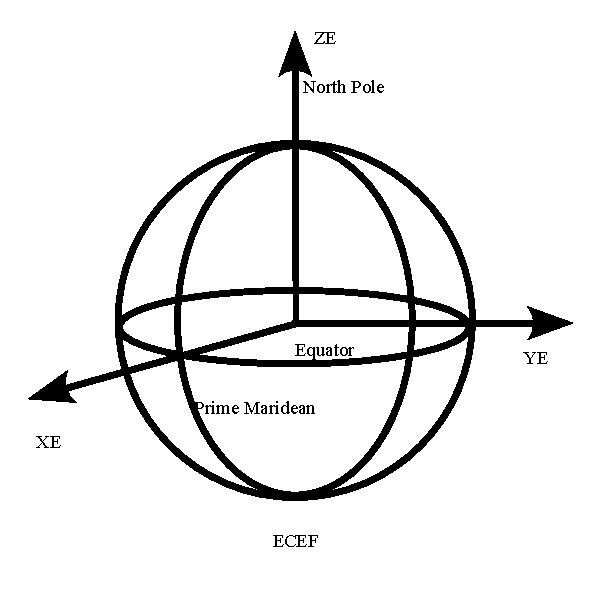
\includegraphics[width=0.5\textwidth]{figures/modelling/ECEF.pdf}
    \caption{The Earth-Centered, Earth-Fixed (ECEF) reference frame, a Cartesian coordinate system fixed relative to the Earth, with its origin at the Earth's center of mass. The $\bar{x}$-axis points toward the intersection of the equator and the prime meridian, the $\bar{y}$-axis points 90° east of the X-axis along the equator, and the $\bar{z}$-axis aligns with the Earth's rotational axis toward the North Pole. This frame is commonly used for satellite navigation, geodesy, and Earth observation applications.}
\end{figure}

%===============================================================================================================================================================
\mysubsection{Earth Centered Inertial}{Earth Centered Inertial}

\noindent The Earth-Centered Inertial (ECI) reference frame, denoted by $\mathcal{I}$, shares its origin with the Earth-Centered Earth-Fixed (ECEF) frame 
but differs in orientation due to the Earth's rotation. While the $\bar{z}$-axis remains aligned with the Earth's rotation axis (pointing toward the North Pole), the $\bar{x}$-axis 
of the ECI frame points toward the Vernal Equinox—the intersection of the Earth's equatorial plane and the ecliptic plane—while the $\bar{y}$-axis completes the right-hand rule. 
Unlike the ECEF frame, which rotates with the Earth, the ECI frame is non-rotating with respect to the distant stars, making it suitable for orbital dynamics and space 
navigation. The transformation from ECEF to ECI is governed by Earth's rotation about its $\bar{z}$-axis at an angular velocity of $\omega_e = 7.2921 \times 10^{-5}~\text{rad/s}$, 
resulting in a rotation of $\theta = \omega_e t$ over time $t$.
\vspace{0.5cm}

\noindent Closely related to the ECI frame is the International Celestial Reference Frame (ICRF), particularly the J2000 realization, which serves as a 
quasi-inertial reference frame for astronomical and space applications. The ICRF is defined by the positions of distant extragalactic radio sources, such as quasars, 
which are so far away that they appear fixed relative to Earth's motion, providing an extremely stable reference. The J2000 frame is aligned with the Earth's 
mean equator and equinox at the epoch J2000.0 (January 1, 2000, 12:00 TT) and is the standard frame for expressing the positions and motions of celestial bodies, 
satellite orbits, and spacecraft attitudes, especially in deep-space navigation.
\vspace{0.5cm}

\noindent To transform from the ECEF to the ECI fame the following DCM is constructed by

\begin{equation}
    \mathbf{A}_{\mathcal{R}}^{\mathcal{I}} = R(\omega_e t) = 
    \begin{bmatrix}
        \cos(-\omega_e t) & -\sin(-\omega_e t) & 0\\
        \sin(-\omega_e t) & \cos(-\omega_e t) & 0\\
        0 & 0 & 1
    \end{bmatrix}
    \text{, and}
\end{equation}

\begin{equation}
    \mathbf{T}_\mathcal{R}^\mathcal{I} =
    \begin{bmatrix}
    \mathbf{A}_\mathcal{R}^\mathcal{I} & \mathbf{0}_{3\times1} \\
    \mathbf{0}_{1\times3} & 1 \\
    \end{bmatrix}
\end{equation}

\begin{figure}[H]
    \centering
    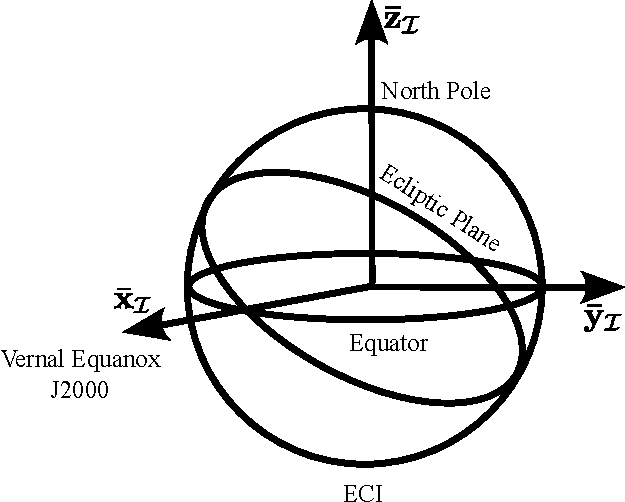
\includegraphics[width=0.6\textwidth]{figures/modelling/ECI.pdf}
    \caption{The Earth-Centered Inertial (ECI) reference frame, an inertial Cartesian coordinate system with its origin at the Earth's center of mass. Unlike Earth-fixed frames, the ECI frame does not rotate with the Earth, making it suitable for describing the motion of satellites, spacecraft, and other celestial objects relative to the stars. It provides a consistent reference for orbital mechanics and space navigation.}
    \label{fig:3.11}
\end{figure}

%=======================================================================================================================================================================
\mysubsection{Orbital Reference Frame}{Orbital Reference Frame}

The orbital reference frame used is the Local Vertical Local Horizon (LVLH) denoted by $\mathcal{O}$. The LVLH frame is a rotating, orbit-attached corrdinate
system commonly used in spacecraft dynamics. It moves with the satellite and is defined relative to its orbit around Earth. The $\bar{z}$-axis is the local vertical and is 
also called the Nadir direction, it points to the barycenter of the system, in this case the center of the Earth. The $\bar{y}$-axis is called the cross track that points 
out of the orbital plane, typically the anti-angular momentum vector direction (anti-normal to the orbit plane). The $\bar{x}$-axis is the "Local Horizon" also called
"along track" pointing forward it is tangent to the orbit and completes the right hand rule.
\vspace{0.5cm}

\noindent If $\mathbf{r}_\mathcal{I}$ is the position vector of the satellite and $\mathbf{v}_\mathcal{I}$ is the velocity vector of the satellite.
The reference frame unit vectors are determined by:

\begin{align}
    \mathbf{\bar{z}}_{\mathcal{O}} &= -\frac{\mathbf{r}_\mathcal{I}}{||\mathbf{r}_\mathcal{I}||}\text{,} \\
    \mathbf{\bar{y}}_{\mathcal{O}} &= \frac{\mathbf{r}_\mathcal{I}\times\mathbf{v}_\mathcal{I}}{||\mathbf{r}_\mathcal{I}\times\mathbf{v}_\mathcal{I}||}\text{, and}\\
    \mathbf{\bar{x}}_{\mathcal{O}} &= \mathbf{\bar{y}}_{\mathcal{O}}\times\mathbf{\bar{z}}_{\mathcal{O}}
\end{align}

\noindent This reference frame also requires a translation and is performed by

\begin{equation}
    \mathbf{A}_{\mathcal{I}}^{\mathcal{O}} = 
    \begin{bmatrix}
            \mathbf{\bar{x}}_{\mathcal{O}} \\
            \mathbf{\bar{y}}_{\mathcal{O}} \\
            \mathbf{\bar{z}}_{\mathcal{O}}
    \end{bmatrix}
    \text{, and}
\end{equation}

\begin{equation}
    \mathbf{T}_{\mathcal{I}}^{\mathcal{O}} = 
    \begin{bmatrix}
            \mathbf{A}_{\mathcal{I}}^{\mathcal{O}} & -\mathbf{A}_{\mathcal{I}}^{\mathcal{O}}\mathbf{r}_\mathcal{I} \\
            \mathbf{0}_{1\times3} & 1\\
    \end{bmatrix}
\end{equation}

\begin{figure}[H]
    \centering
    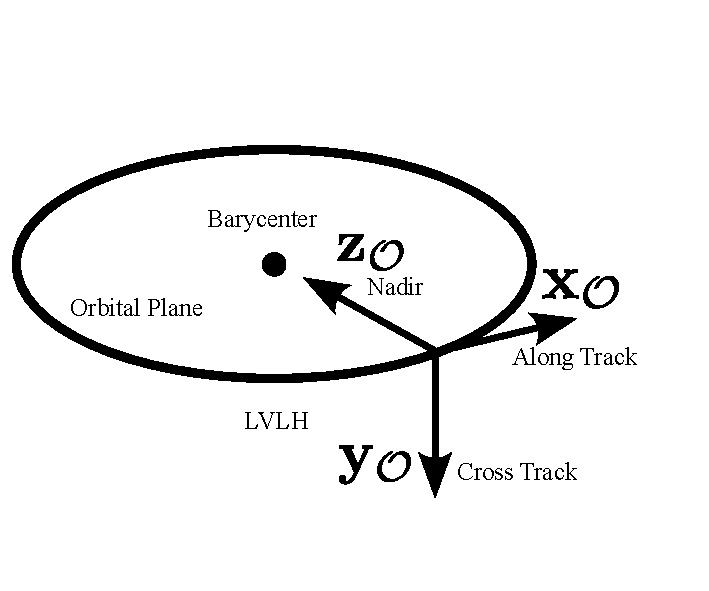
\includegraphics[width=0.7\textwidth]{figures/modelling/LVLH.pdf}
    \caption{The Orbital Reference Frame, also known as the Local Vertical Local Horizontal (LVLH) frame, is a spacecraft-centered coordinate system used to describe positions and orientations relative to an orbiting body. Its origin is at the spacecraft's center of mass, the $\bar{z}$-axis points toward the center of the Earth (nadir), the $\bar{y}$-axis is aligned opposite to the orbital angular momentum vector (orbit normal), and the $\bar{x}$-axis completes the right-handed system, pointing along the velocity vector in the orbital plane. This frame is widely used in attitude control, guidance, and navigation for satellites.}
    \label{fig:3.6}
\end{figure}


%=======================================================================================================================================================================
\mysubsection{Body Referenece Frame}{Body Referenece Frame}

The body reference frame denoted by $\mathcal{B}$ is the reference frame of the satellite body itself, with the center point referenced as the center of mass of the satellite 
body with the $\bar{z}$-axis defined as the yaw, $\bar{x}$-axis defined as the roll and the $\bar{y}$-axis defined as the pitch of the satellite as illustrated in Figure \ref{fig:BRF}. Converting from one reference frame to another 
a DCM needs to be constructed from the true attitude $\mathbf{q}_\mathcal{B/O}$ like in Equation \ref{Eq:3.10}

\begin{equation}
    \mathbf{A}_\mathcal{O}^\mathcal{B} = f(\mathbf{q}_\mathcal{B/O})
    \text{, and}
\end{equation}

\begin{equation}
    \mathbf{T}_\mathcal{O}^\mathcal{B} =
    \begin{bmatrix}
    \mathbf{A}_\mathcal{O}^\mathcal{B} & \mathbf{0}_{3\times1} \\
    \mathbf{0}_{1\times3} & 1 \\
    \end{bmatrix}
    \text{.}
\end{equation}

\begin{figure}[H]
    \centering
    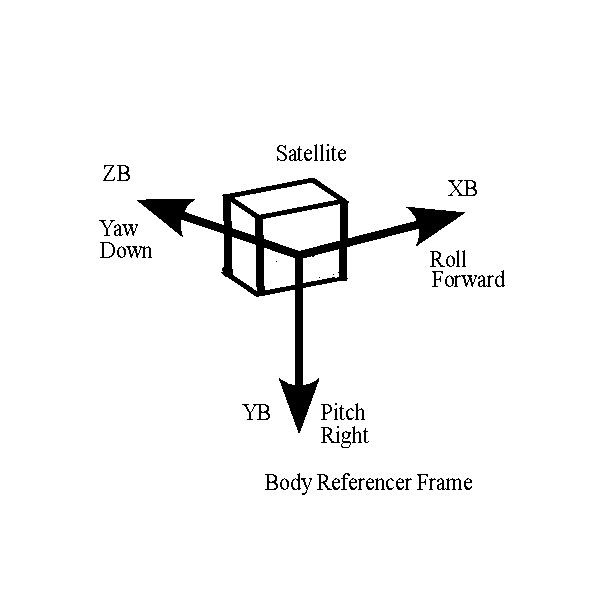
\includegraphics[width=0.5\textwidth]{figures/modelling/BRF.pdf}
    \caption{The Body Reference Frame, denoted by $\mathcal{B}$, is fixed to the satellite itself, with its origin at the satellite’s center of mass. The axes are defined relative to the satellite's orientation: the $\bar{x}$-axis corresponds to roll, the $\bar{y}$-axis to pitch, and the $\bar{z}$-axis to yaw.}
    \label{fig:BRF}
\end{figure}

%==================================================================================================================================================================
\mysubsection{North - East - Down/ East - North - Up }{East - North - Down/ East - North -Up}

The North-East-Down (NED) and East-North-Up (ENU) reference frames are not promanant refrence frames in this work, but it is worth a mention
as it is used in sensor modeling and system initialization. Both frames are defined at a specific location by the geodetic latitude $\phi$, longitude $\lambda$, 
and altitude $h$. The ENU frame has axes pointing East, North, and Up, whereas the NED frame has axes pointing North, East, and Down as we can see in Figure \ref{fig:ENU}
The transformation from the Earth-Centered Earth-Fixed (ECEF) frame to the ENU frame is:

\begin{equation}
\mathbf{A}_\mathcal{R}^{\mathcal{E}} =
\begin{bmatrix}
-\sin\lambda & \cos\lambda & 0 \\
-\sin\phi\cos\lambda & -\sin\phi\sin\lambda & \cos\phi \\
\cos\phi\cos\lambda & \cos\phi\sin\lambda & \sin\phi
\end{bmatrix}
\label{eq:ecef2enu}
\text{.}
\end{equation}

\noindent Similarly, the transformation from the ECEF frame to the NED frame is:

\begin{equation}
\mathbf{A}_\mathcal{R}^{\mathcal{N}} =
\begin{bmatrix}
-\sin\phi\cos\lambda & -\sin\phi\sin\lambda & \cos\phi \\
\cos\lambda & \sin\lambda & 0 \\
-\cos\phi\cos\lambda & -\cos\phi\sin\lambda & -\sin\phi
\end{bmatrix}
\label{eq:ecef2ned}
\text{.}
\end{equation}

\begin{figure}[H]
    \centering
    \includegraphics[width=0.5\textwidth]{figures/modelling/NED.pdf}
    \caption{The East-North-Up refrence frame}
    \label{fig:ENU}
\end{figure}


%=========================================================================================================================================================================
\mysection{Sensor Modelling}{Sensor Modelling}
\label{sec:SensorModelling}

\noindent
To properly model the satellite sensors, it is necessary to define the \textbf{truth state vector} $\mathbf{x}_\text{true}$, which represents the complete, ideal state of the satellite. All sensor measurements are simulated relative to this true state. The truth state includes the satellite's position and velocity in the Earth-Centered Inertial (ECI) frame, its orientation as a quaternion describing the rotation from the orbital frame to the body frame, and its angular velocity relative to the orbital frame:

\begin{equation}
\begin{split}
\mathbf{r}_{\mathcal{I},\text{true}} &= [x_\text{position}, y_\text{position}, z_\text{position}]^T, \\
\mathbf{v}_{\mathcal{I},\text{true}} &= [x_\text{velocity}, y_\text{velocity}, z_\text{velocity}]^T, \\
\mathbf{q}_{\mathcal{B/O},\text{true}} &= [s_\text{attitude}, x_\text{attitude}, y_\text{attitude}, z_\text{attitude}]^T, \\
\boldsymbol{\omega}_{\mathcal{B/O},\text{true}} &= [x_\text{angular velocity}, y_\text{angular velocity}, z_\text{angular velocity}]^T.
\end{split}
\end{equation}

The full truth state vector is then composed as

\begin{equation}
\mathbf{x}_\text{true} = [\mathbf{r}_{\mathcal{I},\text{true}}, \mathbf{v}_{\mathcal{I},\text{true}}, \mathbf{q}_{\mathcal{B/O},\text{true}}, \boldsymbol{\omega}_{\mathcal{B/O},\text{true}}]^T.
\end{equation}

\noindent
Here, $\mathbf{r}_{\mathcal{I},\text{true}}$ and $\mathbf{v}_{\mathcal{I},\text{true}}$ describe the satellite's exact position and velocity in the ECI frame, $\mathbf{q}_{\mathcal{B/O},\text{true}}$ specifies its true orientation as a quaternion, and $\boldsymbol{\omega}_{\mathcal{B/O},\text{true}}$ represents the angular velocity of the satellite body relative to the orbital reference frame.


%=========================================================================================================================================================================
\mysubsection{GPS Sensor Model}{GPS Sensor Model}
\label{sec:GPSModel}

In simulation, GPS measurements are generated using the same underlying orbital dynamics as the true satellite model, based on the two-body problem. This ensures consistency between the satellite’s true motion and its simulated sensor data. To emulate realistic sensor characteristics, Gaussian noise and drift are introduced into the measurements.
\vspace{0.5cm}

\noindent The GPS measurement model is given by:
\begin{equation}
    \mathbf{z}_{GPS,\mathcal{R}}(t) = \mathbf{r}_{\mathcal{R},\text{true}}(t) + \boldsymbol{\eta}_{GPS}(t) + \mathbf{d}_{GPS}(t),
\end{equation}

\noindent where $\mathbf{z}_{GPS}(t)$ is the measured position at time $t$. It is expressed as the sum of the true satellite position $\mathbf{r}_{\mathcal{R},\text{true}}(t)$, propagated through the two-body dynamics, additive zero-mean Gaussian noise $\boldsymbol{\eta}_{GPS}(t)$, and a drift term $\mathbf{d}_{GPS}(t)$ accounting for long-term bias.

\begin{equation}
    \begin{split}
        \mathbf{r}_{\mathcal{R},\text{true}}^+ &= \mathbf{T}_\mathcal{I}^\mathcal{R} \times \mathbf{r}_{\mathcal{I},\text{true}}^+ \\
    \end{split}
\end{equation}

\noindent The drift term models the slow, cumulative error typical of low-cost GPS receivers. It follows a random walk process:
\begin{equation}
    \mathbf{d}_{GPS}(t) = \mathbf{d}_{GPS}(t - \Delta t) + \mathbf{q}_{GPS}(t),
\end{equation}

\noindent where $\mathbf{d}_{GPS}(t - \Delta t)$ is the previous drift value, and $\mathbf{q}_{GPS}(t)$ is a mean-zero random increment representing the drift rate, typically sampled from a Gaussian distribution:
\begin{equation}
    \mathbf{q}_{GPS}(t) \sim \mathcal{N}(0, \sigma_d^2 \mathbf{I}).
\end{equation}

\noindent This formulation captures both short-term variability through $\boldsymbol{\eta}_{GPS}(t)$ and long-term bias accumulation via $\mathbf{d}_{GPS}(t)$, resulting in a more realistic sensor simulation for estimation performance testing.
\vspace{0.5cm}

\noindent GPS outputs are typically provided in standard NMEA message formats such as the \$GPGGA sentence, which includes time, latitude, longitude, and altitude. To produce equivalent measurements in simulation, the ECEF-frame output $\mathbf{z}_{GPS,\mathcal{R}}(t)$ is transformed to geodetic coordinates $\mathcal{L}$ (latitude, longitude, altitude) using the WGS84 reference model, as shown in Figure~\ref{fig:gps}. The resulting groundtrack visualization is given in Figure~\ref{fig:GPS}.

\begin{equation}
    \mathbf{z}_{GPS,\mathcal{L}}(t) = f(\text{WGS84}, \mathbf{z}_{GPS,\mathcal{R}}(t))
\end{equation}

\begin{figure}[H]
    \centering
    \begin{subfigure}{0.45\textwidth}
        \centering
        \includegraphics[width=\linewidth]{figures/modelling/GPS2.pdf}
        \caption{GPS measurement in $\mathcal{L}$ coordinates.}
        \label{fig:gps-a}
    \end{subfigure}
    \hfill
    \begin{subfigure}{0.45\textwidth}
        \centering
        \includegraphics[width=\linewidth]{figures/modelling/GPS3.pdf}
        \caption{Zoomed-in view showing measurement noise.}
        \label{fig:gps-b}
    \end{subfigure}
    \caption{GPS measurement and noise model derived from the $\mathbf{x}_{\text{true}}$ state in the $\mathcal{L}$ reference frame.}
    \label{fig:gps}
\end{figure}

\begin{figure}[H]
    \centering
    \includegraphics[width=0.8\textwidth]{figures/modelling/GPS.pdf}
    \caption{Groundtrack representation of the simulated GPS measurements, illustrating the apparent Earth rotation as the satellite completes an orbit.}
    \label{fig:GPS}
\end{figure}

%=========================================================================================================================================================================
\mysubsection{Gyroscope Sensor Model}{Gyroscope Sensor Model}
\label{sec:GyroModel}

The gyroscope measures the angular velocity of the satellite body frame relative to the inertial frame, expressed in the body frame, denoted as $\boldsymbol{\omega}^B_{B/I}$. This measurement is essential for attitude determination and control.
\vspace{0.5cm}

\noindent To reflect realistic performance, the simulated gyroscope output includes both random noise and time-varying bias (drift), modeled as:
\begin{equation}
    \mathbf{z}_{\text{Gyro}}(t) = \boldsymbol{\omega}^B_{B/I}(t) + \boldsymbol{\eta}_{\text{Gyro}}(t) + \mathbf{d}_{\text{Gyro}}(t),
\end{equation}

\noindent where $\mathbf{z}_{\text{Gyro}}(t)$ is the measured angular velocity, $\boldsymbol{\eta}_{\text{Gyro}}(t)$ represents zero-mean Gaussian noise, and $\mathbf{d}_{\text{Gyro}}(t)$ models the slow drift bias typical of gyroscopes.

\vspace{0.5cm}
\noindent The true angular velocity $\boldsymbol{\omega}_{\mathcal{B}/\mathcal{I}}$ can be obtained from the simulated state $\mathbf{x}_{\text{true}}$, which contains $\boldsymbol{\omega}_{\mathcal{B}/\mathcal{O}}$. To relate these quantities, the orbital angular velocity $\boldsymbol{\omega}_{\mathcal{O}/\mathcal{I}}$ must first be determined:

\begin{equation}
    \boldsymbol{\omega}_\mathcal{O/I}^\mathcal{O} = -\omega_o\mathbf{\bar{y}}_\mathcal{O}, \quad
    \omega_o = \sqrt{\frac{\mu}{r^3}},
\end{equation}

\noindent where $\omega_o$ is the orbital rate, dependent only on orbital radius for a circular orbit. Expressing this in the body frame gives:

\begin{equation}
    \begin{split}
    \boldsymbol{\omega}_\mathcal{O/I}^\mathcal{B} &= \mathbf{A}_\mathcal{O}^\mathcal{B} \times \boldsymbol{\omega}_\mathcal{O/I}^\mathcal{O} \\
    &= 
    \begin{bmatrix}
        -a_{1,2}\omega_o \\
        -a_{2,2}\omega_o \\
        -a_{3,2}\omega_o
    \end{bmatrix}.
    \end{split}
\end{equation}

\noindent The total body angular velocity is then obtained as:
\begin{equation}
    \boldsymbol{\omega}_\mathcal{B/I} = \boldsymbol{\omega}_\mathcal{B/O} + \boldsymbol{\omega}_\mathcal{O/I}.
\end{equation}

\noindent The gyroscope bias evolves according to a random walk model:
\begin{equation}
    \mathbf{d}_{\text{Gyro}}(t) = \mathbf{d}_{\text{Gyro}}(t - \Delta t) + \mathbf{q}_{\text{Gyro}}(t),
\end{equation}

\noindent where $\mathbf{q}_{\text{Gyro}}(t)$ is a random increment drawn from:
\begin{equation}
    \mathbf{q}_{\text{Gyro}}(t) \sim \mathcal{N}(0, \sigma_g^2 \mathbf{I}),
\end{equation}

\noindent with $\sigma_g^2$ denoting the variance of the gyroscope drift rate.
\vspace{0.5cm}

\noindent This model effectively represents both high-frequency noise and long-term bias drift, enabling realistic simulation of Inertial Measurement Unit (IMU) performance. Incorporating these dynamics into the estimation process supports robust attitude and rate reconstruction in the presence of sensor imperfections.

\vspace{0.5cm}
\noindent Figure~\ref{fig:GYRO} illustrates the simulated gyroscope output, showing rotation about the body $z$-axis at approximately $10^\circ/s$, with the combined effects of measurement noise and sampling rate visible in the resulting signal variance.

\begin{figure}[H]
    \centering
    \includegraphics[width=\textwidth]{figures/modelling/GYRO.pdf}
    \caption{Simulated gyroscope measurement showing high-frequency noise and drift.}
    \label{fig:GYRO}
\end{figure}


%==========================================================================================================================================================================
\mysubsection{Coarse Sun Sensor Model}{Coarse Sun Sensor Model}
\label{sec:CSSModel}

The Coarse Sun Sensor (CSS) is a fundamental attitude sensing instrument in nanosatellite systems, providing an estimate of the Sun direction relative 
to the satellites body frame.
\vspace{0.5cm}

\noindent The Sun vector is modeled in the Earth-Centered Inertial (ECI) frame as a fixed unit vector pointing in the $\textbf{X}+$ direction:

\begin{equation}
    \mathbf{S}_\mathcal{I} = \begin{bmatrix} 1 & 0 & 0 \end{bmatrix}^\top
\end{equation}

\noindent This simplified model assumes that the Sun direction does not vary during the simulation.
\vspace{0.5cm}

\noindent To simulate the Sun vector in the satellite's body frame, the inertial vector is rotated using the satellite's true attitude quaternion. 
The corresponding direction cosine matrix (DCM) is derived as:

\begin{equation}
     \mathbf{S}_\mathcal{B}^+ = \mathbf{T}_\mathcal{O}^\mathcal{B} \times \mathbf{T}_\mathcal{I}^\mathcal{O} \times \mathbf{S}_\mathcal{I}^+
\end{equation}

\noindent where $\mathbf{T}_\mathcal{I}^\mathcal{O}$ is the transformation matrix from the inertial to orbit frame and $\mathbf{T}_\mathcal{O}^\mathcal{B}$ is the
transformation from the orbital frame to the body frame.
\vspace{0.5cm}

\noindent The CubeSat is equipped with six coarse sun sensors, one on each face, aligned along the $\pm X$, $\pm Y$, and $\pm Z$ body 
axes (see Figure~\ref{fig:CSS}). Each sensor has a cosine response:

\begin{equation}
     z_i = \max\left(0, \hat{\mathbf{n}}_i^\top \mathbf{S}_\mathcal{B} \right), \quad i = 1, \dots, 6
\end{equation}

\noindent where $\hat{\mathbf{n}}_i$ is the normal vector of the $i$-th sensor surface.

\begin{figure}[H]
    \centering
    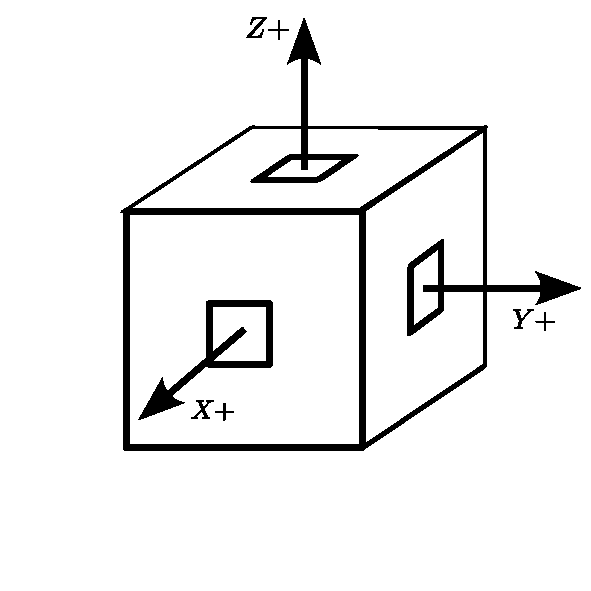
\includegraphics[width=0.4\textwidth]{figures/modelling/CSS.pdf}
    \caption{Orientation of the six coarse sun sensors on the CubeSat}
    \label{fig:CSS}
\end{figure}


\noindent Each CSS reading is perturbed, where \(\boldsymbol{\eta}_{\text{CSS}}\) is a zero-mean 
Gaussian noise vector with covariance \(\mathbf{R}_{\text{CSS}}\):

\begin{equation}
    \mathbf{z}_{\text{CSS}} = \max\left( 0, \mathbf{z}_{\text{CSS}} + \boldsymbol{\eta}_{\text{CSS}} \right)
\end{equation}

\begin{equation}
    \boldsymbol{\eta}_{\text{CSS}} \sim \mathcal{N}(\mathbf{0}, \mathbf{R}_{\text{CSS}}).
\end{equation}

\noindent Negative readings are clamped to zero since physical sensors cannot detect negative intensity.
\vspace{0.5cm}

\noindent The estimated Sun vector in the body frame is reconstructed using a weighted sum of the face normals:

\begin{equation}
    \hat{\mathbf{S}}_\mathcal{B} = \sum_{i=1}^{6} z_i \cdot \hat{\mathbf{n}}_i
\end{equation}

\noindent The result is normalized to produce a unit vector:

\begin{equation}
    \hat{\mathbf{S}}_\mathcal{B} = \frac{\hat{\mathbf{S}}_\mathcal{B}}{|\hat{\mathbf{S}}_\mathcal{B}|}
\end{equation}

\noindent In practice, this sensor is limited by its inability to measure the Sun vector during eclipse conditions, as it requires direct visibility of the Sun. 
However, for the purposes of this project, it is assumed that the Sun remains visible throughout the entire orbit.
\vspace{0.5cm}

\begin{figure}[H]
    \centering
    \includegraphics[width=0.8\textwidth]{figures/modelling/CSSMeasurement.pdf}
    \caption{Simulated CSS measurement illustrating the magnitude of the direction of the sun and the noise.}
    \label{fig:CSSM}
\end{figure}

%=================================================================================================================================================
\mysubsection{Star Tracker Sensor Model}{Star Tracker Sensor Model}
\label{sec:STModel}

The Star Tracker (ST) is a high-accuracy attitude sensor that provides an absolute measurement of the spacecraft's orientation. The way a star tracker works
is by capturing an image of a star field. This star field produces a pointing vector to a star in the body frame. 
\vspace{0.5cm}

\noindent If we define a star catalogue in the ECI frame as 

\begin{equation}
    \boldsymbol{\Gamma} = \{\mathbf{s}_1, \mathbf{s}_2, \ldots, \mathbf{s}_N\},
\end{equation}

\noindent where each \(\mathbf{s}_i \in \mathbb{R}^3\) is a unit vector pointing towards a known star.
\vspace{0.5cm}

\noindent The measurement in the body reference frame is given by

\begin{equation}
    \mathbf{s}_{i,\mathcal{B}}^+ = \mathbf{T}^\mathcal{B}_\mathcal{O} \times \mathbf{T}^\mathcal{O}_\mathcal{I} \times \mathbf{s}_{i,\mathcal{I}}^+,
\end{equation}

\noindent where \(\mathbf{T}^\mathcal{B}_\mathcal{O}\) and \(\mathbf{T}^\mathcal{O}_\mathcal{I}\) are transformation matrices dependent on the true spacecraft state \(\mathbf{x}_\text{true}\). Figure \ref{fig:ST} illustrated how each star measurement is seen out of the BRF of the satellite
\vspace{0.5cm}

\begin{figure}[H]
    \centering
    \includegraphics[width=0.4\textwidth]{figures/modelling/ST.pdf}
    \caption{Represenstation of star vectors calcualted out of the center of mass of the satellite, each star vector is a unit vector defined in the BRF.}
    \label{fig:ST}
\end{figure}


\noindent The observed star vectors are corrupted by zero-mean Gaussian noise, affecting each component of the vector measurement independently:

\begin{equation}
    \mathbf{z}_{\text{ST},i}(t) = \mathbf{s}_{i,\mathcal{B}}(t) + \boldsymbol{\eta}_{\text{ST},i}(t),
\end{equation}

\noindent where \(\mathbf{z}_{\text{ST},i}(t)\) is the measured star vector at time \(t\) for the \(i^\text{th}\) star, and \(\boldsymbol{\eta}_{\text{ST},i}(t)\) is a zero-mean 
Gaussian noise vector with covariance \(\mathbf{R}_{\text{ST}}\):

\begin{equation}
    \boldsymbol{\eta}_{\text{ST},i}(t) \sim \mathcal{N}(\mathbf{0}, \mathbf{R}_{\text{ST}}).
\end{equation}

\noindent This noise accounts for short-term measurement errors due to sensor resolution, optical distortions, and image processing uncertainties. 
Unlike gyroscope measurements, the star tracker noise does not include a bias or drift term, as star trackers provide absolute attitude references. Figure \ref{fig:STM} shows the simulated measurements of the first four stars in $\Gamma$ and illustrates how the direction changes as the satellite orbits.
\vspace{0.5cm}

\noindent Normally, a star tracker is constrained to the eclipse section of the orbit, as it can only detect stars most precisely in darkness, but in this project it is assumed
that the Star Tracker has a 360° FOV and can see throughout the entire orbit.

\begin{figure}[H]
    \centering
    \includegraphics[width=\textwidth]{figures/modelling/STMeasurement.pdf}
    \caption{Simulated Star Tracker Mesurements from the fisrt 4 Stars, the figure shows how the unit vectors (direction) changes as the satellite orbits.}
    \label{fig:STM}
\end{figure}

%==========================================================================================================================================================================
\mysubsection{Magnetometer Sensor Model}{Magnetometer Sensor Model}

The spacecraft's magnetometer measures the local magnetic field vector at its current position in space. 
This measurement provides both the direction and magnitude of the geomagnetic field, which is essential for attitude determination and control. 
For this project, the magnetic field is modeled using the International Geomagnetic Reference Field (IGRF) defined in the J2000 inertial reference frame. 
The IGRF is a standard mathematical representation of Earth's main magnetic field and its secular variation, commonly used in space applications to ensure 
consistency and accuracy in magnetic field estimation.
\vspace{0.5cm}

\noindent The get the magnetic field vector in ECI, the use of the matlab function \textit{wrldmagm} in the Aerospace toolbox is used. It gives a value in the NED refernce frame
given a specific lattitude longitude and altitude.
\vspace{0.5cm}

\begin{figure}[H]
    \centering
    \includegraphics[width=\textwidth]{figures/modelling/MagneticField.pdf}
    \caption{The total magnetic field intensity given by the \textit{worldmgn} function using IGRF.}
    \label{fig:MagneticField}
\end{figure}


\noindent so first we need to convert the satellites position to LLA using a DCM.

\begin{equation}
    \begin{split}
    \mathbf{r}_\mathcal{R} &= \mathbf{A}_\mathcal{I}^\mathcal{R} \times \mathbf{r}_\mathcal{I} \\
    \mathbf{r}_\mathcal{L} &= f(\text{WGS84},\mathbf{r}_\mathcal{R})        
    \end{split}
\end{equation}

\noindent The position is then provided as an input to the function.

\begin{equation}
    \mathbf{z}_{\text{MAG},\mathcal{N}} = \textit{wrldmagn}[\mathbf{r}_\mathcal{L}, \text{decimalYear}]
\end{equation}

\noindent To get the magnetic field in the body frame we need to transform it with the transformation matrices.

\begin{equation}
    \mathbf{z}_{\text{MAG},\mathcal{B}}^+ = \mathbf{T}_\mathcal{O}^\mathcal{B} \times \mathbf{T}_\mathcal{I}^\mathcal{O} \times \mathbf{T}_\mathcal{R}^\mathcal{I} \times
    \mathbf{T}_\mathcal{N}^\mathcal{R} \times \mathbf{z}_{\text{MAG},\mathcal{N}}^+ 
\end{equation}


\noindent The magnetometer measurement is affected by zero-mean Gaussian noise representing sensor inaccuracies such as electronic noise and environmental disturbances. 
The noisy measurement in the body frame can be expressed as

\begin{equation}
    \mathbf{z}_{\text{MAG},\mathcal{B}}(t) = \mathbf{z}_{\text{MAG},\mathcal{B}}(t) + \boldsymbol{\eta}_{\text{MAG}}(t),
\end{equation}

\noindent where the \(\boldsymbol{\eta}_{\text{MAG}}(t)\) is a zero-mean Gaussian noise vector with covariance \(\mathbf{R}_{\text{MAG}}\):

\begin{equation}
    \boldsymbol{\eta}_{\text{MAG}}(t) \sim \mathcal{N}(\mathbf{0}, \mathbf{R}_{\text{MAG}}).
\end{equation}

\noindent This noise models the short-term fluctuations and measurement errors inherent to magnetometer sensors and does not include any long-term bias or drift, assuming 
that calibration and compensation are applied as illustrated in Figure \ref{fig:MagM}.

\begin{figure}[H]
    \centering
    \includegraphics[width=0.8\textwidth]{figures/modelling/MagM.pdf}
    \caption{Simulated Magnetoemeter measurements indicating the magnetific field strength in nT and which direction it is measured in according to the IGRF.}
    \label{fig:MagM}
\end{figure}

%==============================================================================================================================================================
\mysection{Conclusion}{Conclusion}
\label{sec:modconclusion}

\noindent
This chapter presented the complete modelling framework of the satellite system, encompassing the orbital dynamics, attitude kinematics, and sensor representations. The two-body dynamics model provided the foundation for simulating the satellite's motion, while the attitude model described the rotational behaviour through quaternion-based propagation. Furthermore, the inclusion of sensor models such as the star tracker, magnetometer, accelerometer, and GPS enabled realistic measurement simulations that reflect the practical constraints of on-orbit systems. Together, these components established a coherent and physically consistent platform upon which the remainder of the study is built.
\vspace{0.5cm}

\noindent
Beyond defining the mathematical relationships, the modelling process also clarified how system assumptions and simplifications influence downstream performance. The accuracy of these models directly affects the realism of the simulated imagery and the reliability of the estimated states. In this context, the modelling stage functions not merely as a theoretical formulation, but as a crucial factor influencing the accuracy and interpretability of the subsequent results.
\vspace{0.5cm}

\noindent
The next chapter, Image Processing (Chapter \ref{chap:imgpros}), builds upon this framework to extract spatial and temporal information from the simulated imagery, while State Estimation (Chapter \ref{chap:stateestimation}) integrates these processed measurements into a unified estimation architecture. 

%=================================================================================================================================================================
